\documentclass[11pt,a4paper]{article}

\usepackage[utf8]{inputenc}
\usepackage[T1]{fontenc}
\usepackage[italian]{babel}
\usepackage{graphicx}
\usepackage{amsmath}
\usepackage{booktabs}
\usepackage{hyperref}
\usepackage{geometry}
\usepackage{caption}
\geometry{margin=2.5cm}

\hypersetup{
    colorlinks=true,
    linkcolor=blue,
    urlcolor=blue,
    citecolor=blue
}

\title{Previsione dell'abbandono clienti (Customer Churn)\\
\large Progetto del corso Introduzione al Pensiero Computazionale e alla Data Science}
\author{Alessia \and Michelle}
\date{\today}

\begin{document}

\maketitle

\begin{abstract}
Questo report presenta un'analisi del dataset \emph{Customer Churn}, relativo a clienti di un'azienda di telecomunicazioni, con l'obiettivo di individuare i fattori associati all'abbandono del servizio e di costruire modelli predittivi in grado di identificare i clienti a rischio. Vengono confrontati tre modelli di classificazione (Regressione Logistica, k-Nearest Neighbors, Random Forest) e discussi i risultati alla luce dello squilibrio tra le classi e dell'interpretabilità di ciascun approccio. Il codice sorgente e i notebook completi sono disponibili nel repository GitHub del progetto: \url{https://github.com/ale19ssia/progetto-data-science}.
\end{abstract}

\section{Introduzione}

L'abbandono dei clienti (\emph{churn}) è uno dei problemi più comuni affrontati dalle aziende che operano con un modello di business ad abbonamento, come le compagnie di telecomunicazioni. Prevedere in anticipo quali clienti sono a rischio di abbandono permette di intervenire con azioni mirate di fidelizzazione, riducendo i costi legati all'acquisizione di nuovi clienti.

L'obiettivo di questo progetto è duplice: da un lato comprendere quali caratteristiche dei clienti sono più associate all'abbandono attraverso un'analisi esplorativa dei dati; dall'altro costruire e confrontare diversi modelli di classificazione in grado di prevedere la variabile target \texttt{Churn} (Sì/No).

Il lavoro è organizzato in sei fasi, seguendo la struttura richiesta dal corso: comprensione del dataset, analisi esplorativa, modellazione, valutazione dei risultati e, infine, questo report. Tutto il codice, i notebook eseguiti e la cronologia dello sviluppo sono disponibili nel repository GitHub del progetto.

\section{Il dataset}

Il dataset utilizzato (\texttt{Customer\_Churn.csv}) contiene informazioni su 7043 clienti di un'azienda di telecomunicazioni, descritti da 21 variabili suddivise in quattro categorie: dati demografici (genere, se cliente anziano, presenza di partner o persone a carico), servizi sottoscritti (telefono, internet, sicurezza online, supporto tecnico, streaming, ecc.), informazioni contrattuali (durata del rapporto in mesi, tipo di contratto, metodo di pagamento, addebiti mensili e totali) e la variabile target \texttt{Churn}.

La variabile target è moderatamente sbilanciata: il 73.5\% dei clienti è rimasto attivo, mentre il 26.5\% ha abbandonato il servizio. Questo squilibrio ha guidato alcune scelte metodologiche descritte nella Sezione~\ref{sec:metodologia}.

Durante la fase di comprensione dei dati è emerso un problema di qualità non evidente a un primo controllo: la colonna \texttt{TotalCharges}, pur rappresentando un importo, era codificata come testo. Analizzando le righe non convertibili in valore numerico, sono stati individuati 11 clienti con un valore vuoto, tutti caratterizzati da \texttt{tenure = 0}, cio\`e clienti appena iscritti e non ancora fatturati. Non si tratta quindi di un errore casuale, ma di un caso sistematico e spiegabile: questi valori sono stati impostati a zero prima della modellazione.

\'E stato inoltre verificato che \texttt{customerID} \`e un identificativo univoco per ogni cliente, privo di valore predittivo, ed \`e stato escluso dalle variabili utilizzate nei modelli.

\section{Metodologia}
\label{sec:metodologia}

\subsection{Preparazione dei dati}

Prima della modellazione, i dati sono stati trasformati come segue: rimozione della colonna identificativa \texttt{customerID}; codifica binaria (0/1) delle variabili con due sole categorie (es. \texttt{Partner}, \texttt{Dependents}, \texttt{PaperlessBilling}); codifica \emph{one-hot} delle variabili con pi\`u di due categorie (es. \texttt{Contract}, \texttt{PaymentMethod}, \texttt{InternetService}). Il dataset \`e stato quindi suddiviso in un training set (75\%) e un test set (25\%), mantenendo la stessa proporzione di clienti che abbandonano in entrambi gli insiemi (\emph{stratified split}). Le variabili numeriche sono state standardizzate (media 0, deviazione standard 1) per i modelli basati sulla distanza o su un'ottimizzazione lineare (Regressione Logistica, k-NN); la standardizzazione non \`e stata applicata per la Random Forest, che non ne necessita.

\subsection{Modelli utilizzati}

Sono stati addestrati e confrontati tre modelli di classificazione, come richiesto dalle specifiche del progetto:

\begin{itemize}
    \item \textbf{Regressione Logistica} (modello lineare): stima la probabilit\`a che un cliente abbandoni come
    \begin{equation}
        P(\text{Churn} = 1 \mid \mathbf{x}) = \frac{1}{1 + e^{-(\beta_0 + \beta_1 x_1 + \cdots + \beta_n x_n)}}
        \label{eq:logistic}
    \end{equation}
    dove $x_1, \ldots, x_n$ sono le variabili standardizzate e $\beta_1, \ldots, \beta_n$ i coefficienti stimati dal modello.
    \item \textbf{k-Nearest Neighbors} ($k=5$, modello non lineare): classifica un cliente in base alla classe maggioritaria tra i 5 clienti pi\`u simili nel training set, secondo la distanza euclidea.
    \item \textbf{Random Forest} (200 alberi, modello non lineare): combina le previsioni di molti alberi decisionali addestrati su sottoinsiemi diversi di dati e variabili.
\end{itemize}

Data la moderata sbilanciatura delle classi, per Regressione Logistica e Random Forest \`e stato utilizzato il parametro \texttt{class\_weight="balanced"}, che assegna un peso maggiore agli esempi della classe minoritaria durante l'addestramento. Il k-NN non dispone nativamente di questo meccanismo.

\subsection{Metriche di valutazione}

Per ciascun modello sono state calcolate: accuratezza (\emph{accuracy}), precisione (\emph{precision}), richiamo (\emph{recall}) e F1-score sulla classe di interesse (\texttt{Churn = S\`i}), oltre alla matrice di confusione. La F1-score \`e definita come la media armonica tra precisione e richiamo:
\begin{equation}
    F_1 = 2 \cdot \frac{\text{precision} \cdot \text{recall}}{\text{precision} + \text{recall}}
    \label{eq:f1}
\end{equation}

Dato lo squilibrio delle classi, l'accuratezza da sola non \`e una metrica sufficiente: un modello che prevedesse sempre ``non abbandona'' otterrebbe gi\`a un'accuratezza del 73.5\% senza fornire alcuna utilit\`a pratica. Per questo motivo \`e stata data particolare attenzione alla recall sulla classe \texttt{Churn}, che misura la capacit\`a del modello di individuare i clienti realmente a rischio.

\section{Risultati}

\subsection{Analisi esplorativa}
\label{sec:eda}

L'analisi esplorativa ha permesso di verificare diverse ipotesi formulate durante la fase di comprensione del dataset. Il fattore pi\`u fortemente associato all'abbandono \`e risultato il tipo di contratto (Figura~\ref{fig:contract}): i clienti con contratto mensile abbandonano nel 42.7\% dei casi, contro l'11.3\% dei contratti annuali e il 2.8\% dei contratti biennali. Anche l'anzianit\`a del cliente (\texttt{tenure}) mostra una relazione marcata con l'abbandono: i clienti che abbandonano hanno una permanenza mediana di 10 mesi, contro i 38 mesi circa di chi resta cliente.

\begin{figure}[htbp]
    \centering
    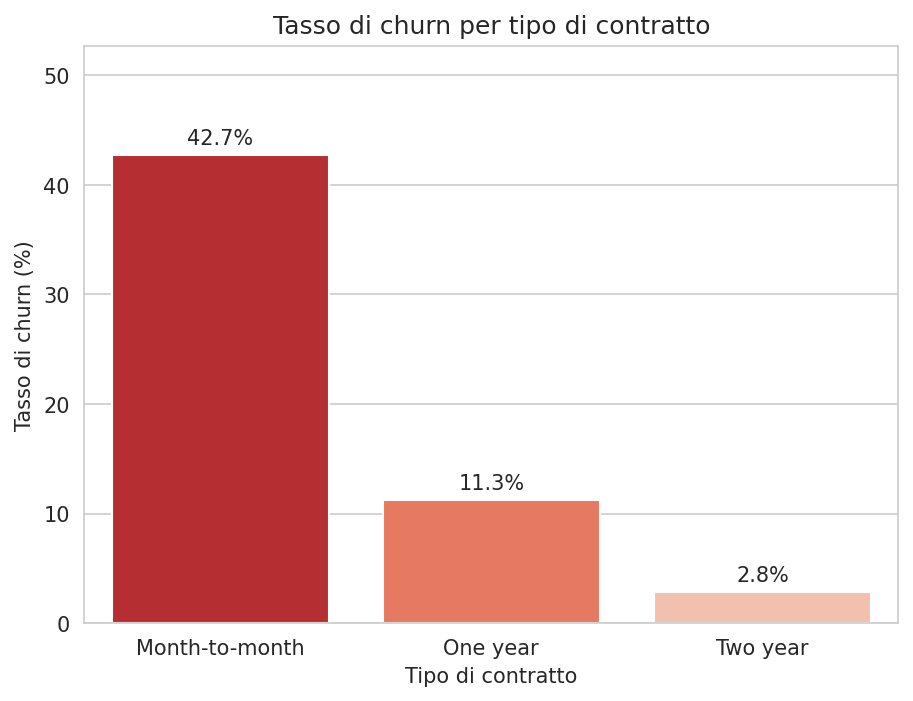
\includegraphics[width=0.75\textwidth]{images/churn_by_contract.png}
    \caption{Tasso di abbandono (\%) per tipo di contratto.}
    \label{fig:contract}
\end{figure}

\'E stata inoltre verificata la presenza di collinearit\`a tra le variabili numeriche del dataset (Figura~\ref{fig:corr}): \texttt{TotalCharges} risulta fortemente correlata sia con \texttt{tenure} (0.83) sia con \texttt{MonthlyCharges} (0.65), un aspetto tenuto in considerazione nell'interpretazione dei coefficienti della Regressione Logistica.

\begin{figure}[htbp]
    \centering
    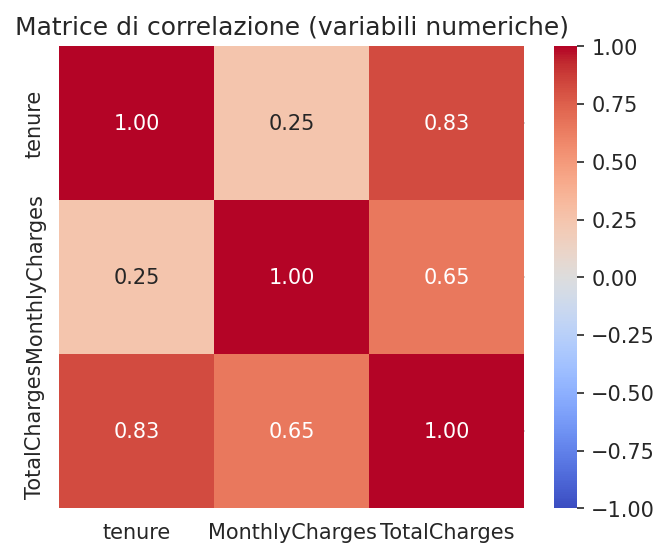
\includegraphics[width=0.55\textwidth]{images/correlation_heatmap.png}
    \caption{Matrice di correlazione tra le variabili numeriche.}
    \label{fig:corr}
\end{figure}

Un'ulteriore ipotesi verificata riguarda il tipo di connessione internet (Figura~\ref{fig:internet}): i clienti con fibra ottica abbandonano nel 41.9\% dei casi, contro il 19.0\% dei clienti con connessione DSL e il 7.4\% di chi non ha internet. La connessione in fibra ottica mostra quindi una forte associazione con il churn, seconda per entit\`a solo al tipo di contratto tra le variabili categoriche esaminate in questa sezione, coerentemente con il coefficiente pi\`u positivo osservato nella Regressione Logistica (Sezione~\ref{sec:importance}).

\begin{figure}[htbp]
    \centering
    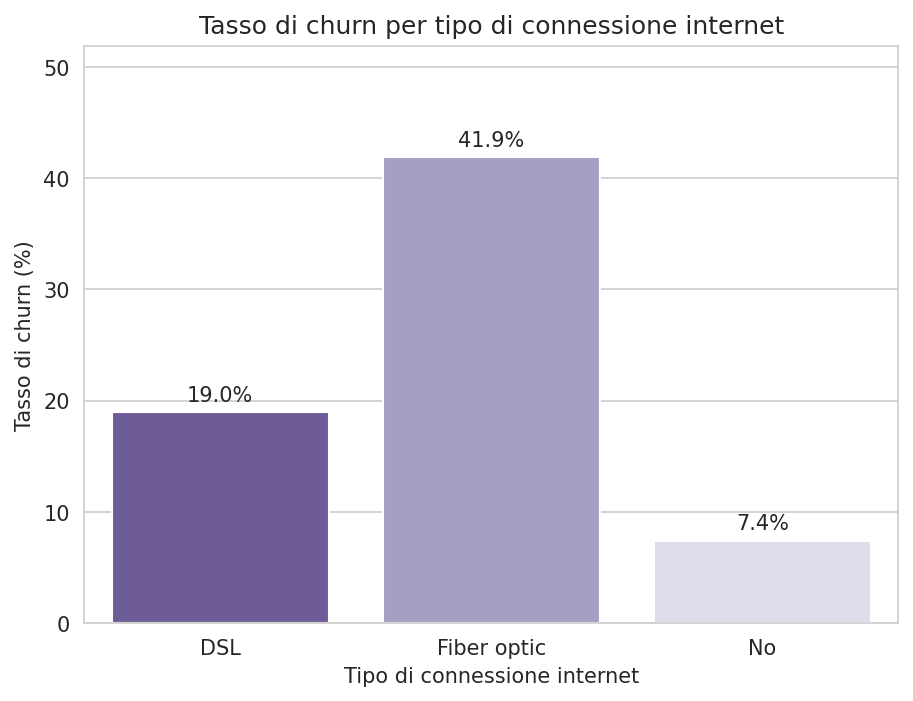
\includegraphics[width=0.75\textwidth]{images/churn_by_internet.png}
    \caption{Tasso di abbandono (\%) per tipo di connessione internet.}
    \label{fig:internet}
\end{figure}

Infine, anche il metodo di pagamento mostra un'associazione con l'abbandono (Figura~\ref{fig:payment}): i clienti che pagano tramite \texttt{Electronic check} abbandonano nel 45.3\% dei casi, contro percentuali inferiori al 20\% per gli altri tre metodi disponibili. Una possibile spiegazione \`e che questo metodo di pagamento sia pi\`u diffuso tra clienti con caratteristiche gi\`a associate al churn, come il contratto mensile; verificare questa ipotesi richiederebbe per\`o un'analisi congiunta delle due variabili, che esula dagli obiettivi di questo report.

\begin{figure}[htbp]
    \centering
    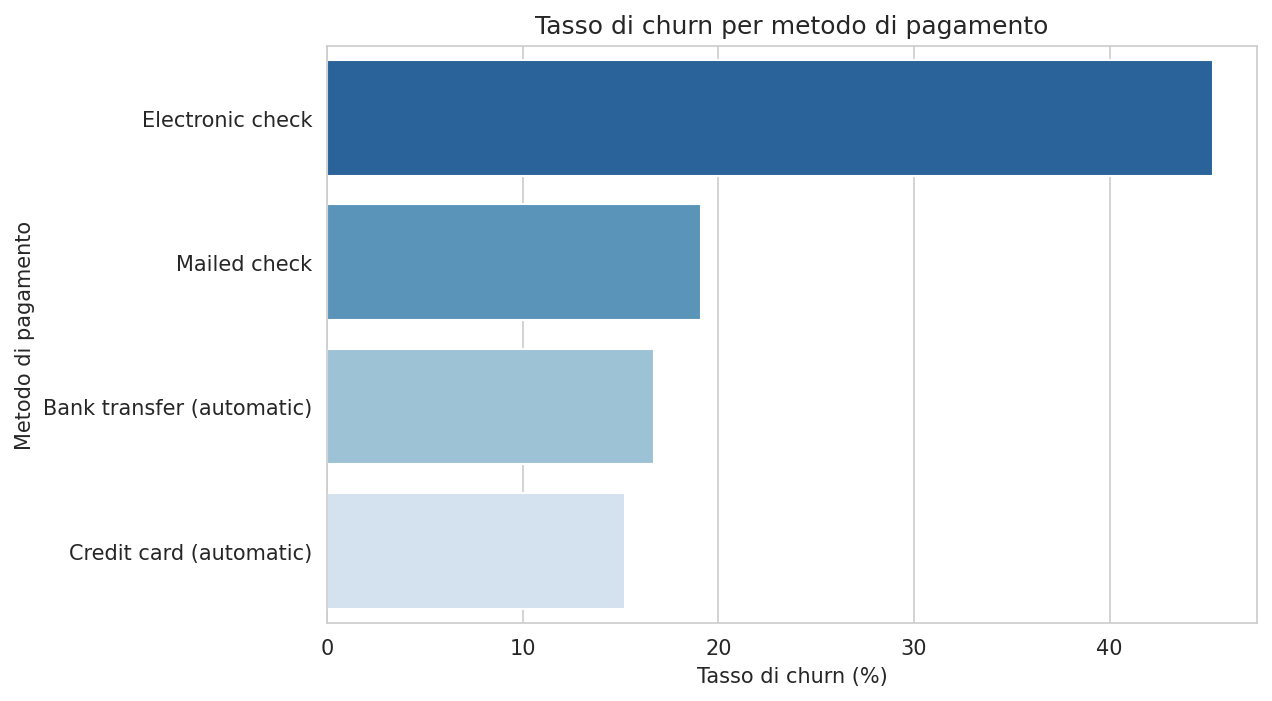
\includegraphics[width=0.75\textwidth]{images/churn_by_payment.png}
    \caption{Tasso di abbandono (\%) per metodo di pagamento.}
    \label{fig:payment}
\end{figure}

\subsection{Confronto tra i modelli}

La Tabella~\ref{tab:results} riporta le metriche di valutazione calcolate sul test set per i tre modelli.

\begin{table}[htbp]
    \centering
    \caption{Confronto delle prestazioni dei tre modelli sul test set (classe \texttt{Churn}).}
    \label{tab:results}
    \begin{tabular}{lcccc}
        \toprule
        \textbf{Modello} & \textbf{Accuracy} & \textbf{Precision} & \textbf{Recall} & \textbf{F1-score} \\
        \midrule
        Regressione Logistica & 0.750 & 0.519 & \textbf{0.797} & \textbf{0.628} \\
        k-Nearest Neighbors   & 0.752 & 0.534 & 0.516 & 0.525 \\
        Random Forest         & \textbf{0.792} & \textbf{0.644} & 0.484 & 0.553 \\
        \bottomrule
    \end{tabular}
\end{table}

La Random Forest raggiunge l'accuratezza e la precisione pi\`u alte, ma \`e la Regressione Logistica a ottenere la recall pi\`u elevata (0.797): individua quindi la quota maggiore di clienti che abbandonano realmente, a fronte di un numero maggiore di falsi positivi. Il k-NN ottiene le prestazioni pi\`u basse tra i tre modelli, coerentemente con l'assenza di un meccanismo di bilanciamento delle classi.

\begin{figure}[htbp]
    \centering
    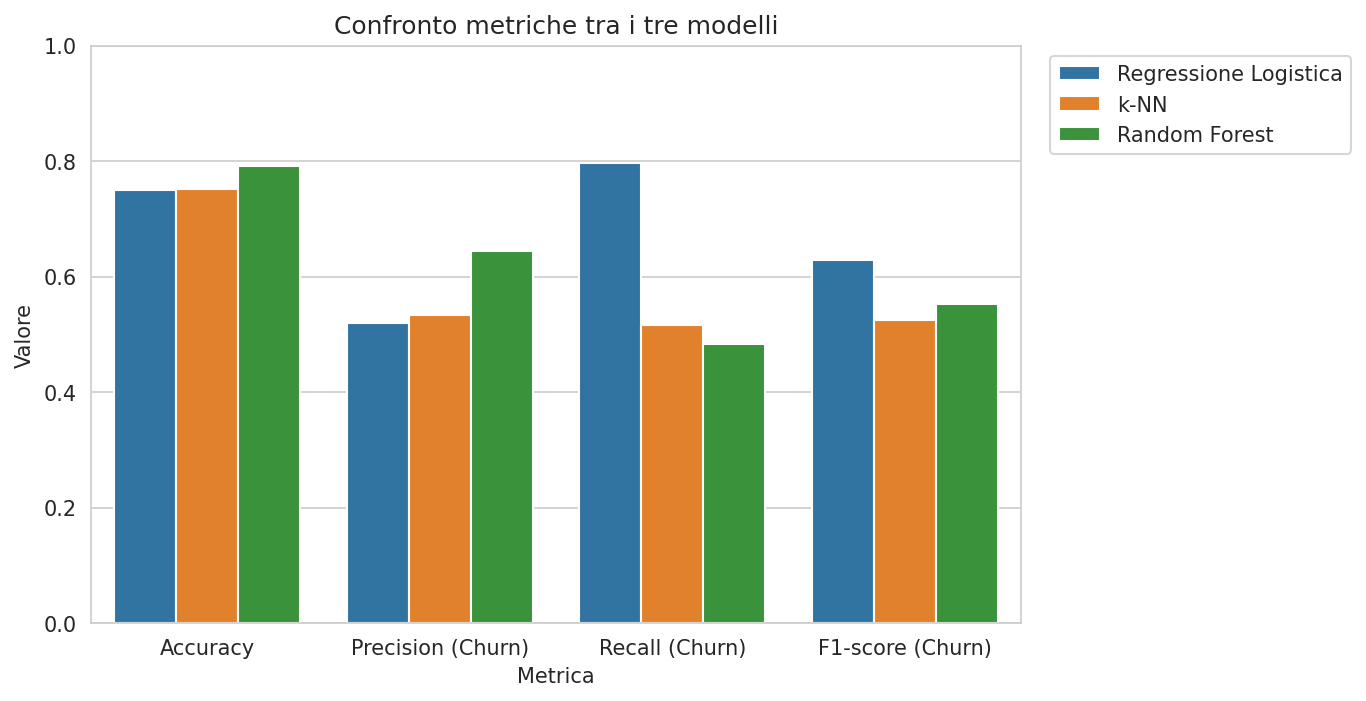
\includegraphics[width=0.8\textwidth]{images/model_comparison.png}
    \caption{Confronto grafico delle metriche di valutazione tra i tre modelli.}
    \label{fig:comparison}
\end{figure}

Le matrici di confusione dei tre modelli (Figura~\ref{fig:cm}) mostrano nel dettaglio la distribuzione degli errori: si nota chiaramente come la Regressione Logistica commetta meno falsi negativi (clienti a rischio non individuati) rispetto agli altri due modelli, a fronte di un numero maggiore di falsi positivi.

\begin{figure}[htbp]
    \centering
    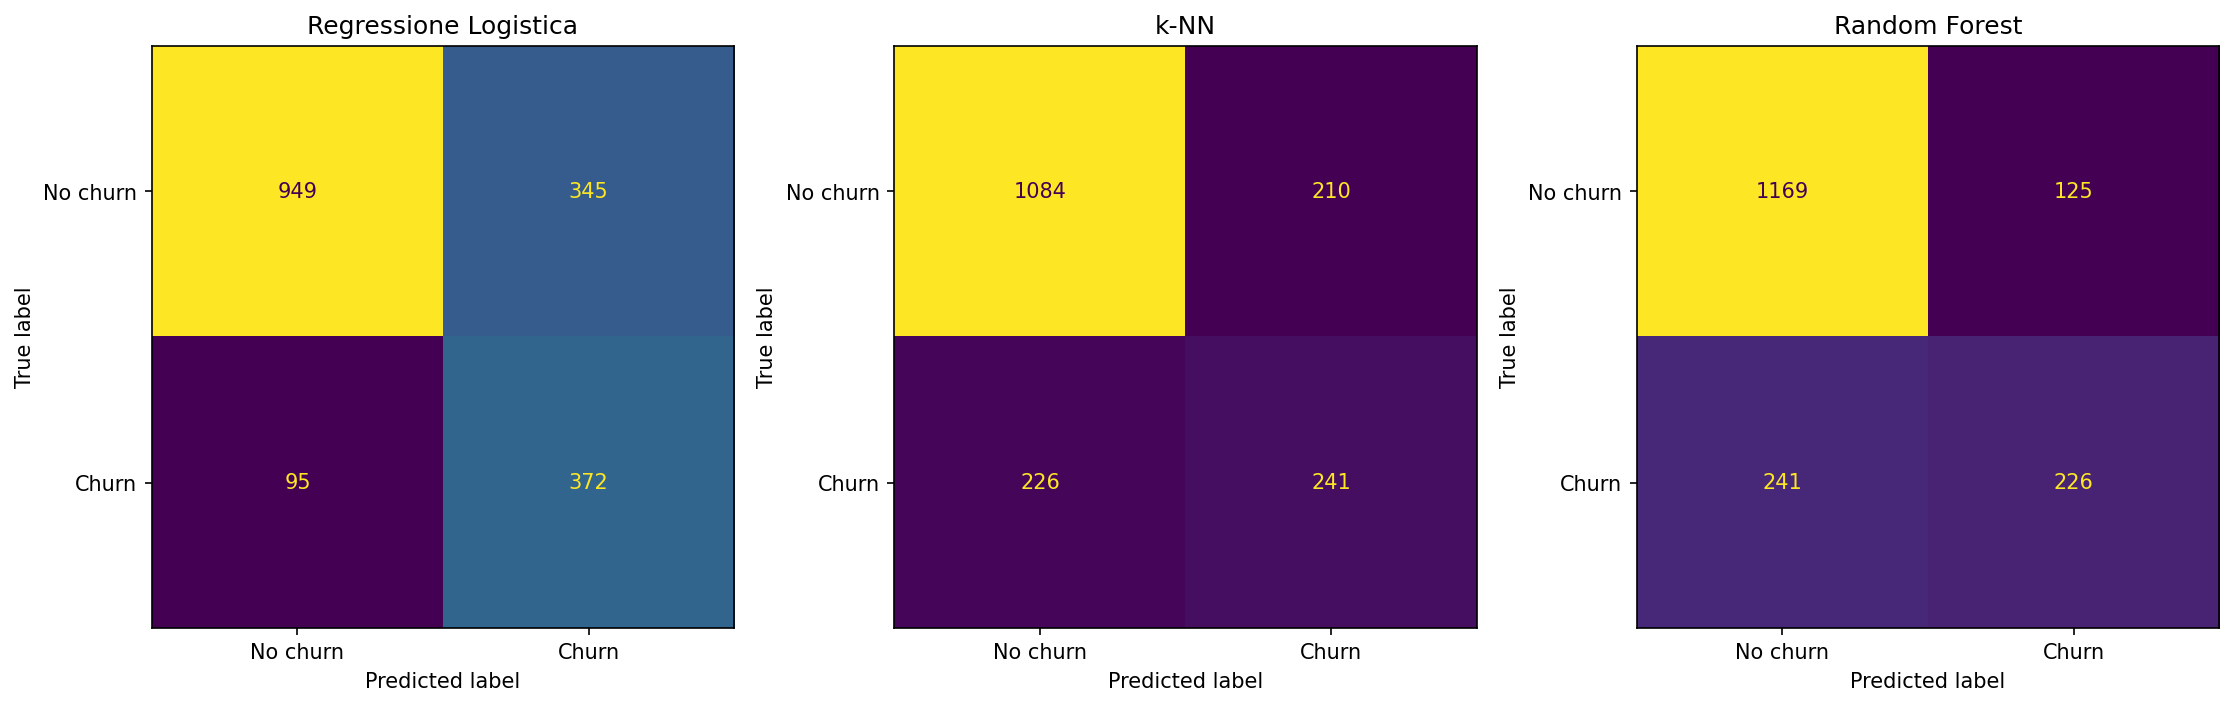
\includegraphics[width=\textwidth]{images/confusion_matrices_confronto.png}
    \caption{Matrici di confusione a confronto per i tre modelli sul test set.}
    \label{fig:cm}
\end{figure}

\subsection{Fattori pi\`u rilevanti}
\label{sec:importance}

La Figura~\ref{fig:importance} mostra le dieci variabili con maggiore \emph{feature importance} secondo la Random Forest. Le tre variabili pi\`u rilevanti sono \texttt{TotalCharges} (0.176), \texttt{tenure} (0.169) e \texttt{MonthlyCharges} (0.150), coerentemente con la collinearit\`a tra queste variabili gi\`a osservata in Sezione~\ref{sec:metodologia}. Il tipo di contratto, pur comparendo pi\`u in basso in questa classifica, resta rilevante: avere un contratto biennale (\texttt{Contract\_Two~year}) \`e la quarta feature per importanza ed \`e anche uno dei coefficienti pi\`u negativi -- quindi pi\`u protettivi -- nella Regressione Logistica. Il coefficiente positivo pi\`u forte nella Regressione Logistica \`e invece \texttt{InternetService\_Fiber~optic} (+0.78), coerente con quanto osservato nell'analisi esplorativa (Sezione~\ref{sec:eda}): i clienti con fibra ottica abbandonano molto pi\`u spesso. Il fatto che due modelli molto diversi tra loro (uno lineare, uno basato su alberi) concordino sui fattori principali rafforza l'affidabilit\`a del risultato.

\begin{figure}[htbp]
    \centering
    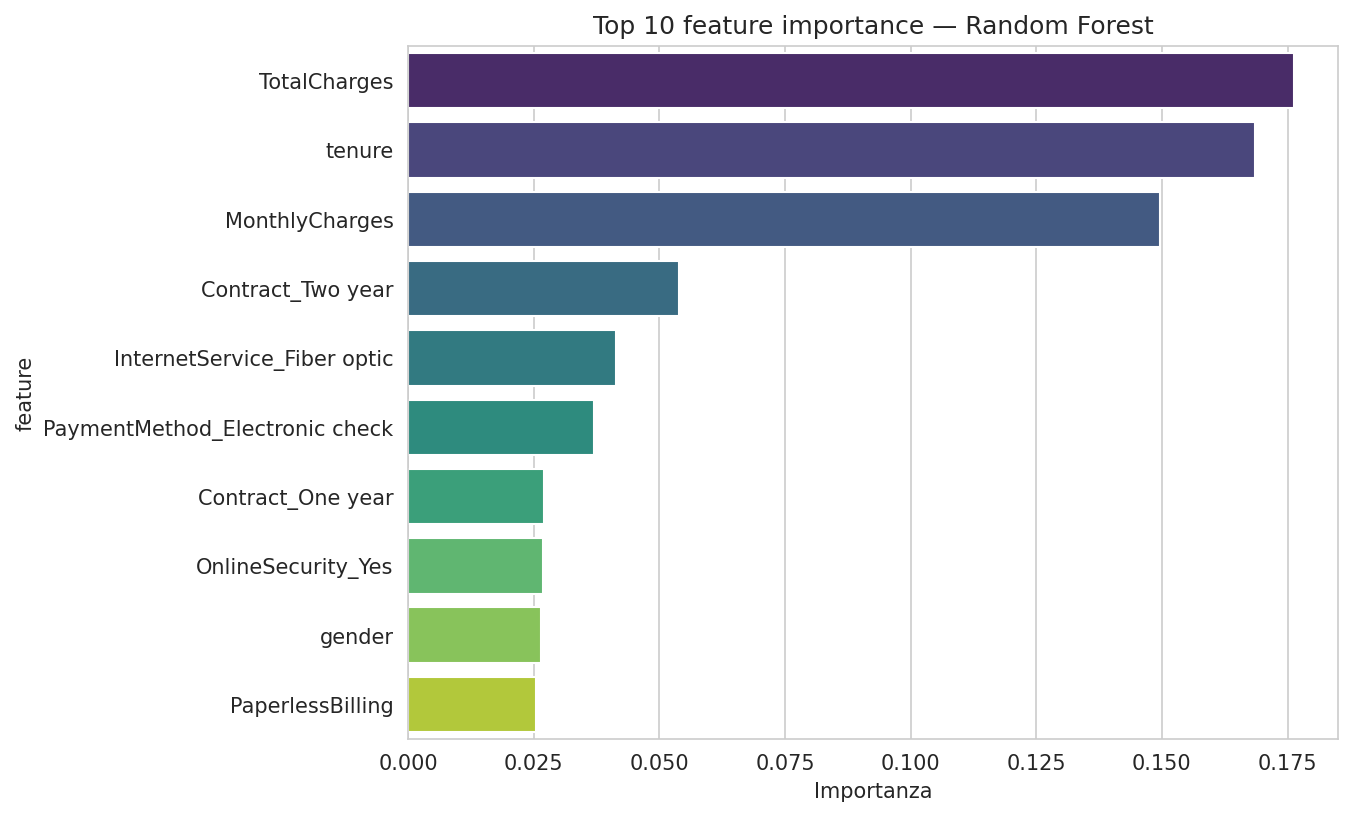
\includegraphics[width=0.75\textwidth]{images/feature_importance_rf.png}
    \caption{Le 10 variabili pi\`u rilevanti secondo la Random Forest.}
    \label{fig:importance}
\end{figure}

\section{Discussione}

I risultati ottenuti evidenziano un compromesso tipico nei problemi di classificazione con classi sbilanciate: la Random Forest privilegia la precisione, mentre la Regressione Logistica, grazie al bilanciamento delle classi, privilegia la recall. Nel contesto applicativo di questo progetto -- identificare clienti a rischio di abbandono per interventi di fidelizzazione -- un falso negativo (un cliente a rischio non individuato) \`e generalmente pi\`u costoso di un falso positivo (un cliente stabile contattato per errore). Su questa base, la Regressione Logistica risulta il modello pi\`u adatto tra i tre, nonostante l'accuratezza pi\`u bassa.

Dal punto di vista dell'interpretabilit\`a, la Regressione Logistica \`e anche il modello pi\`u trasparente: i suoi coefficienti indicano direttamente la direzione e l'intensit\`a dell'associazione stimata tra ciascuna variabile e la probabilit\`a di churn. La Random Forest offre comunque una misura di interpretabilit\`a tramite la feature importance, mentre il k-NN non fornisce alcuna indicazione diretta sull'importanza delle variabili.

Un limite comune a tutti i modelli \`e la precisione relativamente contenuta sulla classe \texttt{Churn} (tra il 52\% e il 64\%): un'azienda che utilizzasse questi modelli per decidere quali clienti contattare dovrebbe considerare che una parte non trascurabile dei clienti segnalati come a rischio in realt\`a non abbandonerebbe. Va inoltre ricordato che la feature importance e i coefficienti stimati indicano associazioni statistiche apprese dal modello, non necessariamente relazioni di causa-effetto.

Dal punto di vista computazionale, la Random Forest (200 alberi) \`e il modello pi\`u oneroso da addestrare, sebbene su un dataset di questa dimensione la differenza rispetto agli altri due modelli sia contenuta a pochi secondi.

\section{Conclusioni}

L'analisi condotta ha permesso di identificare i fattori pi\`u associati all'abbandono dei clienti in un'azienda di telecomunicazioni: il tipo di contratto, l'anzianit\`a del cliente e, in misura minore, il metodo di pagamento e l'addebito mensile. Tra i tre modelli di classificazione confrontati, la Regressione Logistica rappresenta il miglior compromesso tra capacit\`a predittiva (in particolare la recall sulla classe di interesse) e interpretabilit\`a dei risultati, mentre la Random Forest offre l'accuratezza complessiva pi\`u alta.

Come sviluppi futuri, sarebbe utile esplorare tecniche di bilanciamento delle classi pi\`u sofisticate (ad esempio SMOTE), l'ottimizzazione degli iperparametri dei modelli tramite ricerca sistematica (\emph{grid search}), e l'introduzione di nuove variabili derivate (ad esempio il rapporto tra \texttt{TotalCharges} e \texttt{tenure}) per catturare meglio il comportamento dei clienti nel tempo.

\section*{Nota sull'uso di strumenti di intelligenza artificiale}

Il progetto \`e stato realizzato con il supporto di un assistente basato su un modello linguistico (Claude), utilizzato come aiuto alla programmazione e alla spiegazione dei concetti statistici e di machine learning applicati. Tutte le ipotesi, le scelte metodologiche e le interpretazioni dei risultati presentate in questo report sono state discusse e comprese dagli autori. Maggiori dettagli sono disponibili nel README del repository.

\begin{thebibliography}{9}

\bibitem{dataset}
IBM Sample Data Sets, \emph{Telco Customer Churn}. Dataset fornito nell'ambito del corso Introduzione al Pensiero Computazionale e alla Data Science, Universit\`a di Bologna, A.A. 2025/2026.

\bibitem{sklearn}
Pedregosa, F. et al. (2011). \emph{Scikit-learn: Machine Learning in Python}. Journal of Machine Learning Research, 12, 2825--2830.

\bibitem{seaborn}
Waskom, M. L. (2021). \emph{seaborn: statistical data visualization}. Journal of Open Source Software, 6(60), 3021.

\bibitem{corso}
Poggi, F. (2026). \emph{Slide del corso Introduzione al Pensiero Computazionale e alla Data Science}. Dipartimento di Scienze Politiche e Sociali, Universit\`a di Bologna.

\end{thebibliography}

\end{document}
